\begin{figure}[H]
    \centering
    \noindent%
    \begin{minipage}{0.19\textwidth}
        \centering
        Original 
        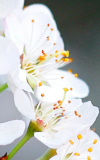
\includegraphics[width=\textwidth]{img/flower/flower.png}
        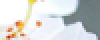
\includegraphics[width=\textwidth]{img/flower/flower-close.png}
    \end{minipage}
    \hfill
    \begin{minipage}{0.19\textwidth}
        \centering
        Bilinear 
        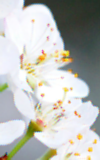
\includegraphics[width=\textwidth]{img/flower/flower-bilinear.png}
        % dcraw -c -q 0 -g 1 1 flower.dng | pnmtopng > flower-bilinear.png
        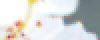
\includegraphics[width=\textwidth]{img/flower/flower-close-bilinear.png}
    \end{minipage}
    \hfill
    \begin{minipage}{0.19\textwidth}
        \centering
        PPG 
        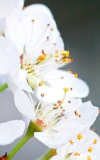
\includegraphics[width=\textwidth]{img/flower/flower-ppg.png}
        % dcraw -c -q 1 -g 1 1 flower.dng | pnmtopng > flower-ppg.png
        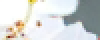
\includegraphics[width=\textwidth]{img/flower/flower-close-ppg.png}
    \end{minipage}
    \hfill
    \begin{minipage}{0.19\textwidth}
        \centering
        VNG 
        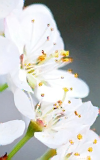
\includegraphics[width=\textwidth]{img/flower/flower-vng.png}
        % dcraw -c -q 2 -g 1 1 flower.dng | pnmtopng > flower-vng.png
        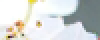
\includegraphics[width=\textwidth]{img/flower/flower-close-vng.png}
    \end{minipage}
    \hfill
    \begin{minipage}{0.19\textwidth}
        \centering
        AHD 
        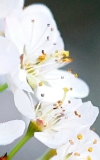
\includegraphics[width=\textwidth]{img/flower/flower-ahd.png}
        % dcraw -c -q 3 -m 3 -g 1 1 flower.dng | pnmtopng > flower-ahd.png
        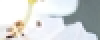
\includegraphics[width=\textwidth]{img/flower/flower-close-ahd.png}
    \end{minipage}
    
    \caption{Visual comparison between different demosaicing algorithms.
    Picture by Hi\'{\^{e}}u Hoàng.
    Present in the images are false colors around the edges of the petals in the bilinear picture, and a reduction in saturation of the stamen on the AHD picture, when compared to the original image.}
    \label{fig:demosiac-comp}
\end{figure}